\documentclass[11pt,a4paper]{article}
\usepackage[utf8]{inputenc}
\usepackage{geometry}
\geometry{margin=1in}
\usepackage{algorithm}
\usepackage{algpseudocode}
\usepackage[hidelinks]{hyperref}
\usepackage{amsmath}
\usepackage{subcaption}

\usepackage{tikz}
\usepackage{tikz}
\usepackage{tikz-3dplot}
\usepackage{array}
\usepackage{pgfplots}
\pgfplotsset{compat=1.18}
\usepackage{pgfplotstable}
\usepackage{adjustbox}
\usetikzlibrary{matrix, shapes.geometric, arrows.meta, positioning, patterns.meta}
\tikzset{
  startstop/.style={rectangle, rounded corners, minimum width=3cm, minimum height=1cm,text centered, draw=black, fill=red!30},
  process/.style={rectangle, minimum width=3cm, minimum height=1cm, text centered, draw=black, fill=blue!20},
  decision/.style={diamond, aspect=2, minimum width=3cm, minimum height=1cm, text centered, draw=black, fill=red!30},
  % cudaKernel_mio/.style={rectangle, minimum width=3cm, minimum height=1cm, text centered, draw=black, fill=green!20},
  subprocess/.style={rectangle, dashed, minimum width=3.5cm, minimum height=1cm, text centered, draw=black, fill=yellow!20},
  cudakernel/.style={
    rectangle, 
    minimum width=3.5cm, 
    minimum height=1cm,
    text centered,
    draw=black, 
    thick,
    fill=green!30,
%    pattern=north east lines,
    pattern color=black
  },
  cudakernel_sub/.style={
    rectangle, 
    dashed,
    minimum width=3.5cm, 
    minimum height=1cm,
    text centered,
    draw=black, 
    thick,
    fill=green!30,
%    pattern=north east lines,
    pattern color=black
  },
  arrow/.style={thick,->,>=Stealth}
}

\title{\textbf{Parallel Computing Project Report:} \textit{Wave Function Collapse}}
\author{Filippo Battisti, Simone Freschet, Francesco Bittasi}
\date{Academic Year 2025/2026}

\usepackage[backend=bibtex, style=numeric]{biblatex}
\addbibresource{refs.bib} 

\begin{document}
\maketitle
\section{Introduction}

Procedural Content Generation (PCG) is a fundamental challenge in computational design, requiring algorithms to produce complex, randomized, yet strictly rule-abiding structures. The Wave Function Collapse (WFC) algorithm, originally introduced by Maxim Gumin in 2016 \cite{gumin2016wave}, elegantly addresses this by framing procedural generation as a formal constraint satisfaction problem. Operating on principles inspired by quantum mechanics, the algorithm initializes a domain where every cell exists in a superposition of all possible states. Through an iterative process of observation and propagation, the algorithm continuously collapses the lowest-entropy cells and strictly enforces adjacency constraints until a globally valid configuration is achieved.

\vspace{1cm}
\begin{figure}[H]
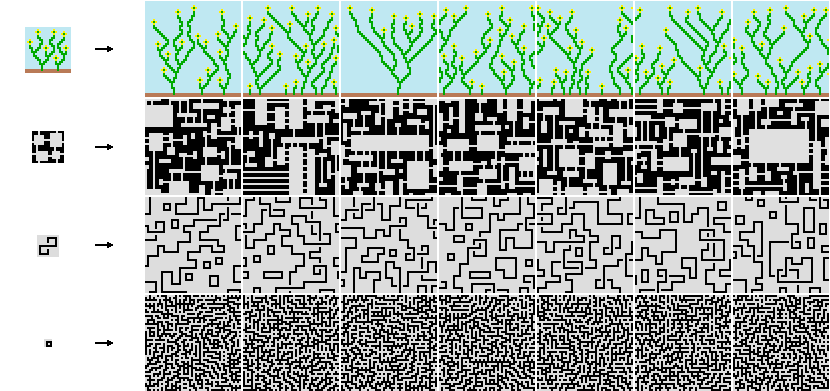
\includegraphics[scale=0.5]{figs/wfc.png}
\caption{Examples from the Maxim Gumin Github repository.}
\end{figure}
\vspace{1cm}

\subsection{Parallel Implementation Challenge}

In recent years, numerous researchers have sought to optimize the computational performance of the WFC algorithm. Notable advancements include the implementation of graph-based data structures to extend WFC beyond rigid spatial grids \cite{kim2019automatic}, as well as the development of hybrid frameworks that combine constraint solving with traditional procedural noise to bypass sequential bottlenecks \cite{buyukcsar2024enhancing}. However, academic literature concerning the direct, distributed parallelization of the core WFC algorithm remains remarkably sparse. This gap is primarily due to the algorithm's inherently non-local constraint propagation: a single cell collapse can trigger a cascading chain reaction of state removals that ripples unpredictably across the entire domain. This creates a highly strict data-dependency structure, where the state of any given cell relies entirely on the successful resolution of constraints originating from distant coordinates. Consequently, true parallel WFC remains a significant and open computational challenge.

To make parallelization feasible, it is strictly necessary to limit the propagation diameter. Once a hard bound on constraint propagation is guaranteed, the computation on a distributed system becomes feasible. In this work, we resolve the sequential bottleneck through a parallel design built upon the Message Passing Interface (MPI). By subdividing the generation domain into nodes and enforcing a policy of exclusive access via mask sliding, we guarantee a conflict-free execution. Crucially, to properly handle the required boundary awareness between adjacent subdomains, our implementation utilizes asynchronous halo-exchange techniques via the MPI interface. This mapping ensures synchronized, overlapping boundary resolution without deadlocks, allowing all nodes to advance in parallel while maintaining the statistical correctness of the final generation.

\subsection{Report Structure}

The remainder of this report is structured as follows. Section 2 details the standard sequential algorithm, establishing the baseline mechanics and strict global data dependencies. Section 3 outlines the parallel design, introducing the conflict-free mask sliding policy. Section 4 presents the topology implementation and the specific tile sets used to limit the propagation bound. Section 5 discusses the technical nuances of the MPI implementation, specifically focusing on domain decomposition, halo exchanges, and centralized data aggregation. Finally, Sections 6, 7, and 8 cover the experimental setup on the CAPRI HPC infrastructure, the execution results, and a critical discussion of the algorithm's scalability limitations and improvements.
\section{Sequential Algorithm}

This section outlines the standard sequential implementation of the Wave Function Collapse algorithm, framing procedural generation as a formal constraint satisfaction problem. By detailing the core observation and propagation loop alongside its computational complexities, we establish the baseline mechanics and highlight the strict global data dependencies that pose challenges for future parallelization.

\subsection{Problem Definition}

The WFC algorithm frames procedural generation as a constraint satisfaction problem. Let the generation domain be a 2D grid $G$ of dimensions $\sqrt{N} \times \sqrt{N}$, containing a total of $N$ cells. 

\begin{itemize}
    \item \textbf{Inputs:} 
    \begin{itemize}
        \item A discrete set of possible tile states or patterns, $T = \{t_1, t_2, \dots, t_k\}$.
        \item A set of adjacency constraints $C$, which dictate whether state $t_a$ can be placed adjacent to $t_b$ in a specific direction $d_{ab} \in \{\text{up, down, left, right}\}$.
        \item A set of weights $W$, representing the frequency or probability of each state appearing.
    \end{itemize}
    
    \item \textbf{State Representation:} Each cell $c_{ij} \in G$ maintains a superposition of currently valid states, denoted as $S_{ij} \subseteq T$ and its entropy $|S_{ij}|$. Initially, the state is completely unobserved, meaning $S_{ij} = T$ for all $c_{ij}$.
    
    \item \textbf{Outputs:} A fully collapsed grid where every cell has exactly one valid state ($|S_{ij}| = 1$), satisfying all constraints in $C$. If any cell's entropy reaches zero, the grid contains an unresolvable contradiction, resulting in a failure state.
\end{itemize}

\subsection{Algorithm and Complexity}
The standard sequential WFC algorithm loops continuously through two primary phases: Observation and Propagation.

\begin{enumerate}
    \item \textbf{Observation:} The algorithm finds the uncollapsed cell (where $|S_{ij}| > 1$) with the lowest entropy to reduce the possibility of future contradictions (zero-entropy states). This phase is implemented with a priority queue extraction to ensure $\mathcal{O}(\log N)$ lookup time. The chosen cell is then collapsed by pseudo-randomly selecting a single state from its remaining superposition, guided by the input weights $W$.
    
    \item \textbf{Propagation:} Once a cell is collapsed, its updated state restricts the valid states of its immediate neighbors. The algorithm recursively propagates these restrictions outward: if a neighbor's superposition is reduced, the propagation continues, and its subsequent neighbors are checked. This cascading chain reaction continues until the neighbor states are no longer affected.
\end{enumerate}

When the whole grid has been collapsed, and thus the priority queue is empty, the execution stops.

\begin{algorithm}[H]
\caption{Sequential Wave Function Collapse}
\begin{algorithmic}[1]
\State \textbf{Input:} Grid $G$ of dimensions $\sqrt{N} \times \sqrt{N}$, Tile set $T$, Constraints $C$ and Weights $W$.
\State \textbf{Output:} Collapsed grid $G$ or \textproc{Failure}
\For{$i,j \gets 0$ to $\sqrt{N}-1$}
    \State $S_{ij} \gets T$
\EndFor
\State $Q \gets G$ \Comment{Add all cells to the priority queue}
\While{$Q.\textproc{NotEmpty}()$}
    \State $c_{min} \gets Q.\textproc{GetMin()}$ 
    \If{$|S_{c_{min}}| = 0$}
        \State \Return \textproc{Failure} \Comment{Contradiction: A cell has 0 possible states}
    \EndIf
    
    \State $t \gets \textproc{RandomState}(W,S_{c_{min}})$
    \State $S_{c_{min}} \gets \{t\}$ \Comment{Collapse the cell to a single state}

    \For{$n \in \textproc{Neighbors}(c_{min})$}
        \State \textproc{Propagate}($c_{min}, n, Q, G, C$)
    \EndFor 
\EndWhile

\State \Return $G$

\vspace{1em}

\Function{Propagate}{$a, b, Q, G, C$}
    \State $d_{ab} \gets$ direction from $a$ to $b$
    \State $Removed \gets \textproc{false}$
    \For{$t \in S_b$}
        \If{no state in $S_a$ allows $t$ based on $C, d_{ab}$}
            \State $S_b \gets S_b \setminus \{t\}$
            \State $Removed \gets \textproc{true}$
        \EndIf
    \EndFor
    \If{$Removed$} \Comment{Neighbor modified, must propagate further}
        \State $Q.\textproc{Update}(b)$ \Comment{Update neighbor's entropy in queue}
        \For{$n \in \textproc{Neighbors}(b) \setminus \{a\}$}
            \State \textproc{Propagate}($b, n, Q, G, C$)
        \EndFor 
    \EndIf
\EndFunction

\end{algorithmic}
\end{algorithm}

\paragraph{Time Complexity} 

Let $|T|$ be the total number of possible states. Across the entire execution of the algorithm, a state can be removed from a cell at most $N \cdot |T|$ times. Processing each removal requires evaluating the constraints against the 4 adjacent neighbors, taking $O(|T|)$ time per neighbor. Therefore, the amortized time complexity of the propagation phase across all iterations is $\mathcal O(N \cdot |T|^2)$. Furthermore, priority queue operations take $\mathcal O(\log N)$ time per update and extraction. Because a cell's priority must be updated each time its entropy drops, which can occur up to $N \cdot |T|$ times, standard implementations yield an overall time complexity of $\mathcal O(N \cdot |T|^2 + N \cdot |T| \log N)$.
    
\paragraph{Space Complexity} The algorithm must store the superposition matrix for the entire grid, which requires $\mathcal{O}(N \cdot |T|)$ space, while the entropy priority queue requires at most $\mathcal{O}(N)$ space. Additionally, evaluating the adjacency constraints using a 3-dimensional bit-matrix (states $\times$ states $\times$ directions) requires $\mathcal{O}(|T|^2)$ space. Therefore, the overall space complexity is bounded by $\mathcal{O}(N \cdot |T| + |T|^2)$.

\paragraph{Data-Dependency Structure}
The core data dependency in WFC lies in the propagation stack. A single collapse at cell $c_{ij}$ can trigger a cascading chain reaction of state removals that ripples across the entire grid $G$. This creates a highly strict, dynamic, and non-local dependency structure: the state of any given cell relies entirely on the successful resolution of constraints originating from completely unpredictable, distant coordinates. This inherently sequential, globally linked constraint propagation is exactly what makes the algorithm difficult to parallelize. As we will see in the following section, however, once a strict limitation in the propagation diameter is determined, a parallel implementation of the algorithm becomes feasible.
\section{Parallel Design}\label{sec:parallel}

Sequential WFC exhibits a strict dependency between successive collapses: each
collapse modifies the superposition set of adjacent chunks, conditioning future
choices. This dependency makes parallelism non-trivial to extract, as a naïve
parallelization in which multiple chunks are collapsed simultaneously without
coordination can produce contradictory states or violate the adjacency
constraints defined by the model.

The approach described here resolves this problem through a decomposition of the
domain into nodes and a policy of exclusive access to chunks via mask sliding,
which guarantees by construction the absence of conflicts between concurrent
collapses. The result is an algorithm in which all nodes advance in parallel
synchronously, each operating in isolation on its own subdomain, with
communications exclusively local to immediate geometric neighbors.

% 1 image representing the mask and chunks

The main properties of the implementation are the following:

\begin{itemize}
    \item \textbf{Statistical correctness:} The parallel output is statistically
    equivalent to the sequential one that is, it belongs to the same distribution
    of valid configurations while not being deterministically identical given the
    same seed, as the global order of collapses differs between the two formulations.

    \item \textbf{Communication locality:} Each node communicates exclusively with
    its immediate geometric neighbors. No global communications are present during
    the collapse phase, with the exception of barrier synchronizations between
    successive slides.

    \item \textbf{Architecture independence:} The adopted parallelism model makes
    no assumptions about the underlying hardware: the decomposition into nodes is
    applicable to distributed-memory systems via MPI, shared-memory systems via
    threads, and hybrid models alike.

    \item \textbf{Conflict-free by construction:} The geometry of the sliding
    guarantees that no chunk is ever covered simultaneously by two distinct masks,
    eliminating the need for locking mechanisms or runtime conflict resolution.
\end{itemize}

For this implementation we define the following elements:

\begin{description}
    \item[Node:] A set of $3 \times 3$ chunks whose evolution is managed by a
    single MPI process or thread. The node is the unit of work of the parallel
    system: it performs the collapse of its own chunks and manages the exchange
    of updates with adjacent nodes.

    \item[Mask:] A $3 \times 3$ chunk window centered on the chunk currently
    being collapsed. It defines the set of chunks that may be influenced by the
    propagation originating from the current collapse, potentially extending onto
    chunks belonging to adjacent nodes.
\end{description}
\begin{figure}[ht]
\centering
\adjustbox{max width=\textwidth}{
\setlength{\fboxsep}{10pt} % imposta il padding a 10pt
\fbox{
\begin{minipage}{0.6\linewidth}
    \centering
    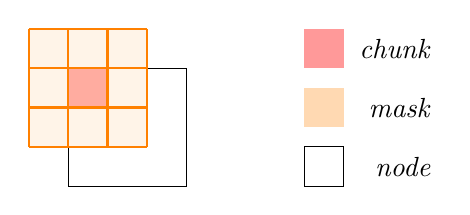
\begin{tikzpicture}[scale=0.5]
    
    \draw[step=1cm, black, thin] (0,0) rectangle (3,3);
    % evidenzio un pixel (0,0)
    \fill[red!40] (0,2) rectangle ++(1,1);
    \fill[orange!30, opacity=0.3] (-1,1) rectangle ++(3,3);
    \draw[step=1cm, orange, thick] (-1,1) grid ++(3,3);
    % legenda
    \fill[color=red!40] (6,3) rectangle ++(1,1);
    \node[anchor=east] at (9.5,3.5) {\textit{chunk}};
    \fill[color=orange!30] (6,1.5) rectangle ++(1,1);
    \node[anchor=east] at (9.5,2) {\textit{mask}};
    \draw[step=1cm, black, thin] (6,0) rectangle ++(1,1);
    \node[anchor=east] at (9.5,0.5) {\textit{node}};
\end{tikzpicture}
\end{minipage}
}}
\caption{Visual representation of chunk, mask and node}
\label{fig:uno}
\end{figure}

\paragraph{Mask sliding and update ordering}
The parallelism of the algorithm is founded on the geometric property by which
the masks of distinct nodes never overlap on the same chunk at the same instant.
To guarantee this property, the mask slides over the 9 chunks internal to the
node following a row-major ordering, visiting positions in sequence from the
bottom row to the top, left to right. At each sliding step, the mask is centered
on a different chunk, and the geometry of the system ensures that the current
chunk is not simultaneously covered by the mask of any adjacent node, making
the local collapse conflict-free.

% 2 image of the sliding masks


\begin{figure}[ht]
\centering
\adjustbox{max width=\textwidth}{
\setlength{\fboxsep}{10pt} 
\fbox{
\begin{minipage}{0.8\linewidth}
    \centering
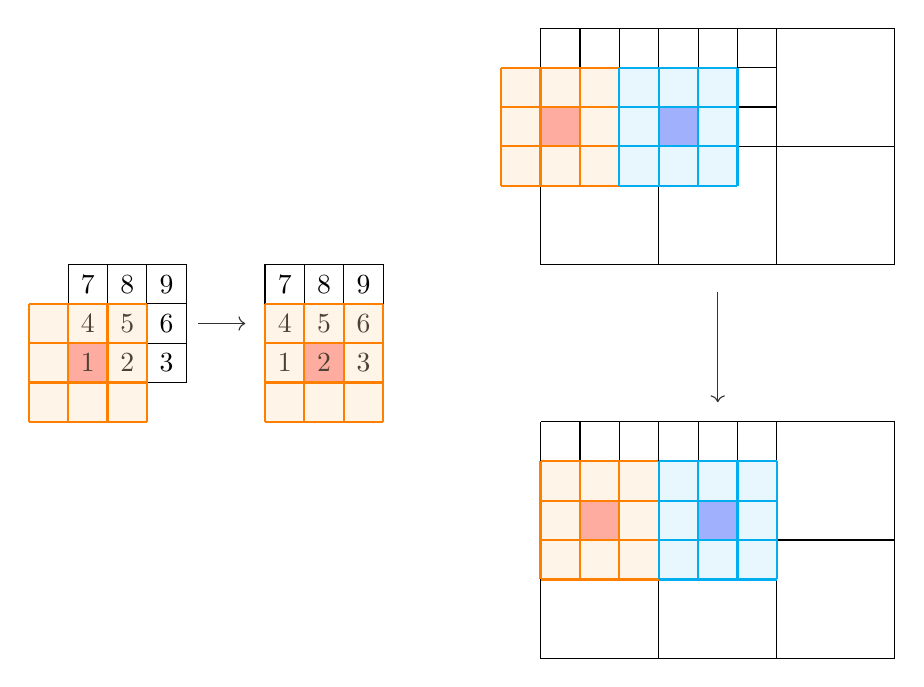
\begin{tikzpicture}[scale=0.5]
    \fill[red!40] (0,-6) rectangle ++(1,1);
    \node at (0.5,-5.5) {1};
    \node at (1.5,-5.5) {2};
    \node at (2.5,-5.5) {3};
    \node at (0.5,-4.5) {4};
    \node at (1.5,-4.5) {5};
    \node at (2.5,-4.5) {6};
    \node at (0.5,-3.5) {7};
    \node at (1.5,-3.5) {8};
    \node at (2.5,-3.5) {9};
    % griglia 7x7
    \draw[step=1cm, black, thin] (0,-6) grid (3,-3);
    % evidenzio un pixel (0,0)
    \fill[orange!30, opacity=0.3] (-1,-7) rectangle ++(3,3);
    \draw[step=1cm, orange, thick] (-1,-7) grid ++(3,3);

    \draw[->, black!80] (3.3,-4.5) -- (4.5,-4.5);

    % griglia 7x7
    \fill[red!40] (6,-6) rectangle ++(1,1);
    \node at (5.5,-5.5) {1};
    \node at (6.5,-5.5) {2};
    \node at (7.5,-5.5) {3};
    \node at (5.5,-4.5) {4};
    \node at (6.5,-4.5) {5};
    \node at (7.5,-4.5) {6};
    \node at (5.5,-3.5) {7};
    \node at (6.5,-3.5) {8};
    \node at (7.5,-3.5) {9};
    \draw[step=1cm, black, thin] (5,-6) grid (8,-3);
    % evidenzio un pixel (0,0)
    \fill[orange!30, opacity=0.3] (5,-7) rectangle ++(3,3);
    \draw[step=1cm, orange, thick] (5,-7) grid ++(3,3);

%% seconda parte !!!!
    \draw[step=1cm, black, thin] (18,0) rectangle (21,3);
    \draw[step=1cm, black, thin] (18,-3) rectangle (21,0);
    \draw[step=1cm, black, thin] (15,-3) rectangle (18,0);
    \draw[step=1cm, black, thin] (12,-3) rectangle (15,0);
    
    \fill[red!40] (12,0) rectangle ++(1,1);
    % griglia 7x7
    \draw[step=1cm, black, thin] (12,0) grid (15,3);
    % evidenzio un pixel (0,0)
    \fill[orange!30, opacity=0.3] (11,-1) rectangle ++(3,3);
    \draw[step=1cm, orange, thick] (11,-1) grid ++(3,3);

    \fill[blue!40] (15,0) rectangle ++(1,1);
    % griglia 7x7
    \draw[step=1cm, black, thin] (15,0) grid (18,3);
    % evidenzio un pixel (0,0)
    \fill[cyan!30, opacity=0.3] (14,-1) rectangle ++(3,3);
    \draw[step=1cm, cyan, thick] (14,-1) grid ++(3,3);

    \draw[->, black!80] (16.5,-3.7) -- (16.5,-6.5);
%% 2.2
\draw[step=1cm, black, thin] (18,-10) rectangle (21,-7);
    \draw[step=1cm, black, thin] (18,-13) rectangle (21,-10);
    \draw[step=1cm, black, thin] (15,-13) rectangle (18,-10);
    \draw[step=1cm, black, thin] (12,-13) rectangle (15,-10);
    \fill[red!40] (13,-10) rectangle ++(1,1);
    % griglia 7x7
    \draw[step=1cm, black, thin] (12,-10) grid (15,-7);
    % evidenzio un pixel (0,0)
    \fill[orange!30, opacity=0.3] (12,-11) rectangle ++(3,3);
    \draw[step=1cm, orange, thick] (12,-11) grid ++(3,3);

    \fill[blue!40] (16,-10) rectangle ++(1,1);
    % griglia 7x7
    \draw[step=1cm, black, thin] (15,-10) grid (18,-7);
    % evidenzio un pixel (0,0)
    \fill[cyan!30, opacity=0.3] (15,-11) rectangle ++(3,3);
    \draw[step=1cm, cyan, thick] (15,-11) grid ++(3,3);

\end{tikzpicture}
\end{minipage}
}}
\caption{Visualization of the mask sliding update order}
\label{fig:due}
\end{figure}

When the mask extends onto chunks belonging to a neighboring node, the owner
node sends a copy of those chunks to the node that needs to update them. The
latter performs the propagation, updates the received copies, and sends them
back to the owner before the next sliding step. The correctness of this exchange
is guaranteed by the fact that, by construction, the owner node does not cover
with its own mask the temporarily transferred chunks, eliminating any access
conflict.

All nodes advance synchronously: each sliding step is preceded by a global
synchronization phase in which each node sends and receives updates relative
to the chunks shared with its neighbors, after which it frees the memory of
chunks no longer needed for the subsequent iteration. Chunks that fall beyond
the boundaries of the global domain are simply ignored.

\subsection{Communication Pattern}
The communication pattern arising from mask sliding is local and point-to-point:
each node communicates exclusively with the geometric neighbors that share a
border or a vertex with it in the node grid.

Communications occur via asynchronous exchange, allowing the internal computation of the node to overlap
with the transfer of boundary data. The volume of data exchanged per
synchronization step is proportional to the number of chunks shared with each
neighbor, the full superposition set of each chunk that is, the set of
compatible patterns for each tile and the thickness of the boundary region
determined by the maximum extent of propagation.



\paragraph{Time Complexity}
Let $P$ be the number of nodes and $L$ the side length of a chunk in tiles.
Each node manages a $3 \times 3$ subdomain of chunks, and its local computation
is equivalent to running sequential WFC on $9 \cdot L^2$ cells. The time
complexity per node is therefore $\mathcal{O}(L^2 \cdot |T|^2 + L^2 |T|\log L)$,
identical to the sequential case scaled to the subdomain size.

Since all nodes advance synchronously and operate in isolation on disjoint
subdomains, the $P$ nodes execute their local computation in parallel, yielding
a parallel time complexity for the computation phase of:
\[
T_{comp}(N,P)=\mathcal{O}\left(\frac NP \cdot |T|^2 + \frac NP|T| \log \frac NP\right)
\]
where $N$ is the total number of cells in the domain. To this must be added
the synchronization overhead $T_{sync}$, incurred at each of the 9 sliding
steps. during which each node exchanges the superposition sets
of the chunks shared with its neighbors.

\[
    T_{sync}(N,P)=\mathcal{O}\left(\frac NP|T|\right)
\] 
In conclusion, the total time complexity for the parallel algorithm is the combination of $T_{comp}$ and $T_{sync}$
$$T(N,P)=T_{comp}(N,P)+T_{sync}(N,P)=\mathcal O\left(\frac NP \cdot |T|^2 + \frac NP |T|\log \frac NP\right)$$

\paragraph{Space Complexity}
Each node stores the superposition states of its $3 \times 3$ chunks, along with temporary copies of boundary chunks received from adjacent nodes. The local memory required to store these chunks is $18 L^2 \cdot |T|$. Combined with the 3-dimensional adjacency bit-matrix, the space complexity per node is $\mathcal{O}(L^2 \cdot |T|+|T|^2)$. Consequently, the total space requirement across all nodes is $\mathcal{O}(N \cdot |T|+P|T|^2)$.



        
\section{Topology-aware implementation}

\subsection{Topologies considered}
[State the topologies you implement and why. Examples (non-exhaustive): linear array, ring, 2D mesh, 2D torus.]

\subsection{Embedding the communication pattern}
[Topology 1]. [How the algorithm's communication maps onto this topology.]

[Topology 2]. [Same as above for the next topology. Highlight the qualitative difference.]

\section{MPI implementation notes}

\subsection{Language and build}
[State the language (C, C++, Rust, Java, Python via mpi4py, \dots) Why this language?]

\subsection{Topology realisation in MPI}
Discuss how each topology is realised and the typical MPI primitives used and justify why.


\section{Experimental setup}

To rigorously evaluate the scalability and efficiency of our parallel Wave Function Collapse implementation, we conducted a series of benchmark experiments. This section details the experimental framework used to validate our architecture. Below, we outline the hardware specifications of the computing environment, define the parameters and methodology guiding our test cases, and describe the specific timing mechanisms used to isolate and measure computational and communication overhead.

\subsubsection{CAPRI infrastructure}
All measurements were conducted on the CAPRI HPC infrastructure of the University of Padua.
Born as a research project to improve the HPC capabilities of the university, differentiating himself from the already available computing resources, this system features:
\begin{itemize}
    \item 16 Intel® Xeon® Gold 6130 CPU (16 cores @ 2.10GHz)
    \item 6 TB DDR4 RAM 
    \item 2 NVIDIA Tesla P100 GPU (3584 Cuda® Cores, 16 GB HBM2)
\end{itemize}

Without considering the GPU's (not used for this project), the CAPRI infrastructure has a theoretical peak performance (FMA single precision) of about 31 TFLOPS.

\subsubsection{Nodes mapping}
The CAPRI infrastructure features an high level abstraction that allows our application to see only one big system with 16 CPU's and 6TB of RAM, considering all CPU's fully interconnected.

The execution of our jobs on the the machine was realized via a SLURM scheduler. For this reason we weren't able to strictly choose the processors and communications used, so we expect some noise from the mapping and the other jobs running on the machine.

\subsection{Methodology}
To observe the average performance of the program, we executed 5 runs with different random seeds (being the running time dependent on randomness) for each configuration of
\begin{itemize}
    \item \textbf{number of processes P}
    \item \textbf{size of the problem L}: the lenght of the side of the image
\end{itemize}
The same 5 seeds were used for each configuration, in this way the problem complexity was proportional to each other and thus the measumements were true indicators of the scalability of the algorithm.

\begin{table}[h!]
\centering
\begin{tabular}{|c|c|}
\hline
\textbf{Parameter} & \textbf{Values} \\
\hline
Problem size $L$ &
$\{1000, 2000, 3000, 4000, 5000, 6000\}$ \\
\hline
MPI processes $P$ &
$\{1, 4, 9, 16, 25, 36, 49, 64\}$ \\
\hline
Seeds $S$ &
$\{123, 456, 789, 1123, 1456\}$ \\
\hline
\end{tabular}
\caption{Experimental parameter space}
\end{table}

Being the jobs queued with respect to the amount of resources required, we scheduled one job for each P. Each job ran all of the 5 runs for each configuration of L.

Having executed all the jobs, python scripts were used to gather the data from the logs and conduct the analysis reported in the next section.

\subsubsection{Measurements}
While for the serial algorithm, the computation wall clock time was measured via the \texttt{clock\_gettime()} function, for the MPI implementation we used the integrated function \texttt{MPI\_Wtime()}: this may cause some differences in the observations made later.

In both cases the rendering time of the image on the output file as been kept out of the measurement: we only observe the total computation time of the algorithm and, in the case of the MPI implementation, we track the time spent in the communications.
The two communication times are obtained measuring the time spent in functions \texttt{MPI\_Sendrecv()} and \texttt{MPI\_Gather()} for each node and then taking the maximum for each run.

\subsubsection{Notes}
While using a shared cluster with SLURM made the process of putting into execution the different tests very easy, the fact that it is a shared platform where big projects are constantly running made it impossible for us to test bigger configurations. At the time of writing, jobs with more than 64 processes have not yet been executed.\

Because of this it's impossible for us to have a complete insight on how the system scales, but we are still able to conduct some useful analysis on the lower "resources-hungry" tests and make some assumptions on how it would perform.
\section{Results}
[Brief description and table and/or plot for each section]

\subsection{Execution time}

\subsection{Speedup and efficiency}

\subsection{Comparison across topologies}

\subsection{Computation vs. communication}

\subsection{Scalability}


\section{Discussion}

With the experimental data established, we now turn to a critical evaluation of the parallel architecture. This discussion interprets the observed scaling efficiency and hardware-bound bottlenecks. Furthermore, it addresses the algorithmic and theoretical limitations of our current tileset design, and outlines actionable strategies for future optimization, specifically targeting the reduction of MPI communication overhead.

\subsection{Comment on the Results}
Looking at the obtained results, we observe that we achieve an optimal speedup as it seems to go develop linearly with the number of processes.
Taking a closer look, even looking at the efficiency statistic, we observe that actually up to 16 processes the algorithm scales super-linearly: this can be explained by the fact that the processes are running on shared local memory and cache and this brings serious advantages.

Once the number of processes cannot be executed on a single socket, as the CAPRI infrastructure only contains cpu's with 16 cores, we observe slowdowns provoked by the time spent in the communication procedures: we see that from P16 to P25 the time pent in synch goes up by about 2 seconds.

This slowdown can be directly observed in the Efficiency study: from P25 the efficiency of our usage of the processors goes down since they spend a lot of time just waiting for the communications. Even with this slowdown the implementations remains efficient in the usage of the different processes since it stops at arount 60\% of usage. 

\subsection{Further Notes on $\texttt{Maze}_{16}$}

In its current formulation, $\texttt{Maze}_{16}$ does not guarantee the global
connectivity of the generated maze: the WFC algorithm may produce multiple
disconnected corridor components that are locally valid with respect to the
tile constraints but do not form a single traversable structure.

Enforcing global connectivity requires a two-phase post-processing pipeline,
which represents the standard approach in procedural content generation for
maze-like environments \cite{atlantis2018pcg}:

\begin{description}
    \item[Flood fill:] Once generation is complete, a flood fill traversal is
    performed from an arbitrary passable cell. All cells reachable from the
    starting point are marked as belonging to the main connected component;
    all remaining passable cells are identified as isolated regions. This step
    runs in $\mathcal{O}(N)$ time and provides a complete map of the
    connectivity structure of the generated maze.

    \item[Selective regeneration:] Isolated regions identified by the flood
    fill are discarded and their cells reset to the virgin state. The WFC
    algorithm is then re-run locally on these regions, with the boundary
    constraints inherited from the surrounding already-collapsed cells, until
    a fully connected configuration is produced.
\end{description}

While this pipeline may appear inefficient due to the potential for repeated
local regenerations, it is consistent with the state of the art in
constraint-based procedural content generation, where post-processing
validation passes are standard practice to enforce global structural
properties that lie outside the scope of local tile
constraints.

The connectivity guarantee was deliberately excluded from the present
implementation: the post-processing pipeline does not interact with the
parallel design in any meaningful way, and no parallel formulation of the
connectivity enforcement step was identified that would not introduce
sufficient synchronization overhead to degrade performance below the
sequential baseline. Although some interesting ideas came up during discussions.

\subsection{Tileset Generalization}
The implementation is designed to accommodate future extensions to additional 
tile sets. The central requirement for any such extension is that the chosen 
tile set must satisfy $\Delta_{prop} < L$, so that propagation remains confined 
within the mask boundary. While this property is amenable to direct proof for 
structured sets such as $\texttt{Maze}_{16}$, no general decision procedure 
exists for establishing $\Delta_{prop}$ for an arbitrary tile set.

This undecidability is a consequence of a deeper result in the theory of Wang 
tiles. Wang conjectured in 1961 that any finite set of tiles capable of tiling 
the plane could do so periodically \cite{wang1961}. His student Robert Berger 
refuted this conjecture in 1966 by proving the undecidability of the domino 
problem that is, no algorithm can determine in general whether a given finite 
tile set admits a valid tiling of the plane constructing as a corollary the 
first known aperiodic tile set \cite{berger1966}. The minimal such set was 
subsequently identified by Jeandel and Rao, who proved that no aperiodic set 
of Wang tiles exists with fewer than 11 tiles or fewer than 4 
colors (where colors are the different types of border connections) \cite{jeandel2015aperiodic}.

As a consequence, no graph-theoretic or structural analysis of an arbitrary 
tile set can decide whether it satisfies the propagation bound required by 
the parallel algorithm. The most practical approach for validating a candidate 
tile set remains probabilistic: a Monte Carlo analysis over a representative 
sample of configurations provides an empirical estimate of $\Delta_{prop}$, 
sufficient for practical purposes even in the absence of a formal proof.


\subsection{Optimizing Data Transfer via Spiral Trajectory and Caching}

Currently, the 9-round mask sliding mechanism evaluates the $3 \times 3$ local grid in a standard row-major order. While geometrically conflict-free, this approach introduces discontinuous jumps in the focal pivot for each round with index multiple of 3.

This overhead can be mitigated by adopting a continuous, spiral-like traversal path together with chunk caching. 
\begin{figure}[H]
\definecolor{m_green}{rgb}{0.1, 0.6, 0.4}
\definecolor{m_red}{rgb}{0.9, 0.2, 0.3}
\centering
\begin{subfigure}[b]{0.48\textwidth}
\centering
\begin{tikzpicture}
    \draw[step=1cm, black, thick] (0,0) grid (3,3);
        
    \draw[->, thick, m_red] (0.5,0.5) -- (2.5,0.5) -- (0.5,1.5) -- (2.5,1.5) -- (0.5, 2.5) -- (2.5, 2.5);

\end{tikzpicture}
\caption{Row Major}
\end{subfigure}
\begin{subfigure}[b]{0.48\textwidth}
\centering
\begin{tikzpicture}
    \draw[step=1cm, black, thick] (0,0) grid (3,3);
        
    \draw[->, thick, m_green] (0.5,0.5) -- (2.5,0.5) -- (2.5,2.5) -- (0.5,2.5) -- (0.5, 1.5) -- (0.5, 1.5) -- (1.5, 1.5);

\end{tikzpicture}
\caption{Spiral}
\end{subfigure}
\caption{The comparison between the current (a) and future (b) round path.}
\end{figure}

Under this configuration, the spatial offset between the pivot at round $k$ and round $k+1$ is strictly bounded to a Chebyshev distance of 1. If we represent the set of chunks covered by the mask at step $k$ as $M_k$, a continuous trajectory maximizes the spatial intersection between consecutive iterations:

$$ |M_k \cap M_{k-1}| = 6 $$

If we introduce a local memory cache for incoming MPI halo data, the node no longer needs to query the full boundary region. Instead, it only needs to fetch the newly exposed frontier:

$$ \Delta M_k = |M_k \setminus M_{k-1}| \le 3 $$

By sliding a cached boundary window, the system requests at most 3 new chunks per iteration. This structural optimization would significantly reduce the overall volume of asynchronous \texttt{MPI\_Sendrecv} data transfers, directly addressing the communication and gathering bottlenecks observed in the strong scaling analysis.



\section{Conclusions}
[5-10 sentences. The headline result and the main lesson learned.]



\printbibliography
\end{document}
